\section{Architecture} % (fold)
\label{sec:architecture}
Figure \ref{fig:dependencygraph} shows the most essential parts of the internal MiCS architecture and how the parts depend on each other. 
This section will describe the different parts, how they relate to one another and how the architecture relates to the five stages outlined in section \ref{sec:workflow_overview}. 

\begin{figure}
	\begin{center}
		\centerline{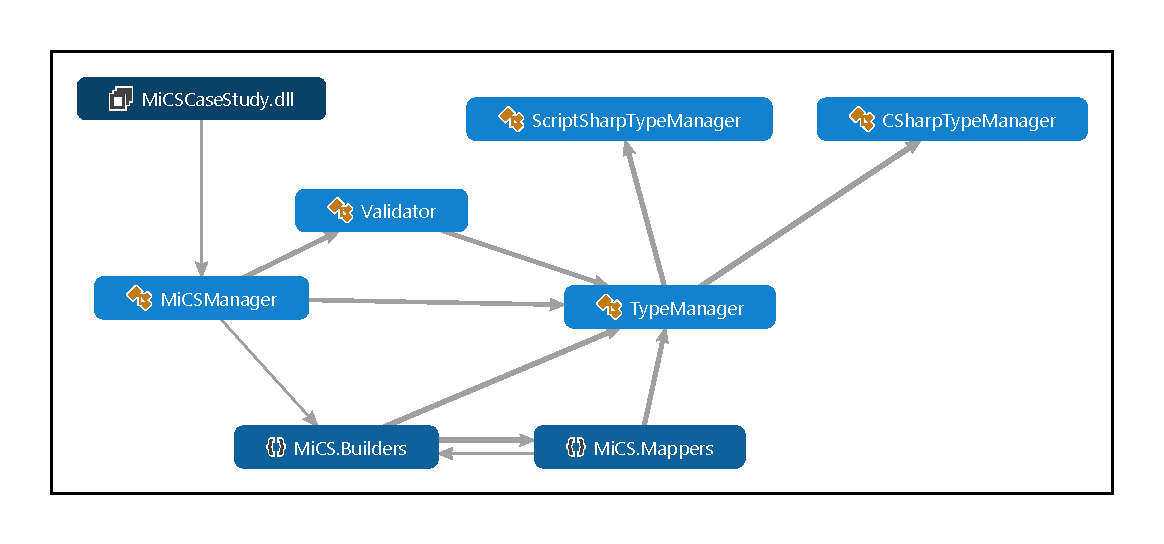
\includegraphics[width=18cm]{resources/images/dependencygraph.pdf}}
	\end{center}
	\caption{The most important parts of the MiCS architecture}
	\label{fig:dependencygraph}
\end{figure}


The TypeManagers (\texttt{TypeManager}, \texttt{CSharpTypeManager} and \texttt{ScriptSharpTypeManager}) provide information about types used throughout MiCS. For example, the TypeManagers are able to look up the type of a symbol (e.g. a variable). Furthermore, they can determine whether a given type is one that the user has defined, or if it is a built-in .NET-type.

The \texttt{Validator} class is responsible for validating the user's code in order to ensure correct type usage before the conversion to Script\# begins.

Classes in the Builders and Mappers namespaces serve as the backbone of MiCS. They are responsible for converting a Roslyn AST to its' corresponding Script\# AST. The Builders traverse the Roslyn AST and builds a corresponding Script\# AST, with help from the Mappers, that handle the actual conversion from Roslyn SyntaxNodes to the corresponding Script\# constructs. (Stage 3)

The \texttt{MiCSManager} class ties the entire MiCS project together and is involved in all of the stages described in section \ref{sec:workflow_overview}. It initializes all the ressource that MiCS needs to function (the TypeManagers) and subsequently initiates all of the processes needed to generate the JavaScript and inject it into the user's web page; first, it starts the validation of the user's code (stage 2). If the validation succeeds, the MiCSManager starts the conversion from Roslyn to Script\# by invoking the Builders (stage 3). When the Script\# AST has been generated, the MiCSManager uses Script\#'s \texttt{ScriptGenerator} to generate the JavaScript source code (stage 4). Lastly, the MiCSManager injects the generated JavaScript into the user's web page by using the pages registered \texttt{ScriptManager} (stage 5). 

% % section architecture (end)